The system consists of five controllers which run in parallel. Each controller is responsible to control its own hardware, communicate with the other controllers and  with the environment. The architecture must be carefully designed in order to satisfy the global requirements defined for the the system (refer to section \ref{sec:global_req}). The most important task of the system is (correctly ordered) delivery of packets, the system being deadlock free and able to use the system to store maximum number of packets possible without increasing complexity of the system. In our design, the maximum number of packets present at any given time in the system is considered to be N, where N is the number of racks. It is however, possible to have $N+1$ packets in the system and still make it work, though this design choice was not considered to keep the design simpler.

It is however not possible to have $N+2$ packets in the system(i.e. packets to be stored on both elevators and $N$ racks at the same time) as it would lead the system into a deadlock/ standstill.

\section*{Description of the controller design}
\subsection*{Controller \textbf{C1}}
This controller is responsible for accepting(or rejecting) an incoming packet from the user, putting the packet on the conveyor belt. It is responsible for controlling the conveyor belt hardware. The required communication must be performed with other controllers to move the packet further into the system.
\subsection*{Controller \textbf{C2}}
This controller is in charge of delivering a packet on request from the user. In addition, it must control the output conveyor belt to move the packet from within the system to the user.
\subsection*{Controller \textbf{C3 and C4}}
These two controllers control their respective elevator hardware. Controller C3, C4 control the upper and lower elevators respectively.
These elevators carry the packets to and from the rack.
\subsection*{Controller \textbf{C5}}
This controller controls the operation of rack(s) in the system. It communicates with all the other controllers to efficiently store the packets onto and retrieve them from the rack.

\begin{figure}[h]
\center
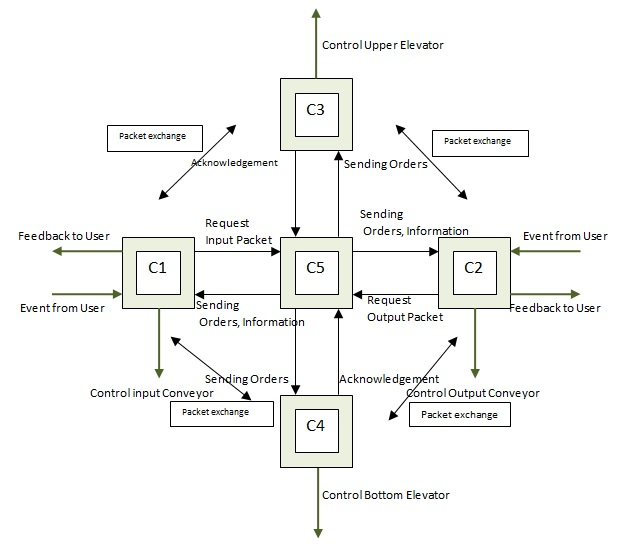
\includegraphics[width=0.7\textwidth]{Architecture_new}
\caption{Architecture of the system}
\label{fig:architecture}
\end{figure}

Figure \ref{fig:architecture} shows the control structure of the system. As seen from the architecture, the controller C5 performs as a master controller that interacts with all the other controllers in the system. 